% mnras_template.tex
%
% LaTeX template for creating an MNRAS paper
%
% v3.0 released 14 May 2015
% (version numbers match those of mnras.cls)
%
% Copyright (C) Royal Astronomical Society 2015
% Authors:
% Keith T. Smith (Royal Astronomical Society)

% Change log
%
% v3.0 May 2015
%    Renamed to match the new package name
%    Version number matches mnras.cls
%    A few minor tweaks to wording
% v1.0 September 2013
%    Beta testing only - never publicly released
%    First version: a simple (ish) template for creating an MNRAS paper

%%%%%%%%%%%%%%%%%%%%%%%%%%%%%%%%%%%%%%%%%%%%%%%%%%
% Basic setup. Most papers should leave these options alone.
\documentclass[a4paper,fleqn,usenatbib]{mnras}

% MNRAS is set in Times font. If you don't have this installed (most LaTeX
% installations will be fine) or prefer the old Computer Modern fonts, comment
% out the following line
\usepackage{newtxtext,newtxmath}
% Depending on your LaTeX fonts installation, you might get better results with one of these:
%\usepackage{mathptmx}
%\usepackage{txfonts}

% Use vector fonts, so it zooms properly in on-screen viewing software
% Don't change these lines unless you know what you are doing
\usepackage[T1]{fontenc}
\usepackage{ae,aecompl}


%%%%% AUTHORS - PLACE YOUR OWN PACKAGES HERE %%%%%

% Only include extra packages if you really need them. Common packages are:
\usepackage{graphicx}	% Including figure files
\usepackage{amsmath}	% Advanced maths commands
\usepackage{amssymb}	% Extra maths symbols
\usepackage{acronym} % Acronyms
\usepackage{siunitx}

%%%%%%%%%%%%%%%%%%%%%%%%%%%%%%%%%%%%%%%%%%%%%%%%%%

%%%%% AUTHORS - PLACE YOUR OWN COMMANDS HERE %%%%%

% Please keep new commands to a minimum, and use \newcommand not \def to avoid
% overwriting existing commands. Example:
%\newcommand{\pcm}{\,cm$^{-2}$}	% per cm-squared

\acrodef{ATNF}[ATNF]{Australia Telescope National Facility}
\acrodef{PHL}[PHL]{Parkes High-Latitude}
\acrodef{PMB}[PMB]{Parkes Multi-Beam}
\acrodef{SMB}[SMB]{Swinburne Intermediate-latitude}

\acrodef{DSS2}[DSS2]{Digital Sky Survey 2}

%%%%%%%%%%%%%%%%%%%%%%%%%%%%%%%%%%%%%%%%%%%%%%%%%%

%%%%%%%%%%%%%%%%%%% TITLE PAGE %%%%%%%%%%%%%%%%%%%

% Title of the paper, and the short title which is used in the headers.
% Keep the title short and informative.
\title[Short title, max. 45 characters]{Práctica 1 - La Vía Láctea con Gaia}

% The list of authors, and the short list which is used in the headers.
% If you need two or more lines of authors, add an extra line using \newauthor
\author[A. Garcia-Garcia et al.]{
A. Garcia-Garcia$^{1}$\thanks{E-mail: agg180@alu.ua.es}
\\
% List of institutions
$^{1}$Grado en Física, Universidad de Alicante\\
}

% These dates will be filled out by the publisher
\date{}

% Enter the current year, for the copyright statements etc.
\pubyear{2020}

% Don't change these lines
\begin{document}
\label{firstpage}
\pagerange{\pageref{firstpage}--\pageref{lastpage}}
\maketitle

% Abstract of the paper
\begin{abstract}

\end{abstract}

% Select between one and six entries from the list of approved keywords.
% Don't make up new ones.
\begin{keywords}
stars: magnetic field -- stars: neutron -- pulsars: general -- methods: observational
\end{keywords}

%%%%%%%%%%%%%%%%%%%%%%%%%%%%%%%%%%%%%%%%%%%%%%%%%%

%%%%%%%%%%%%%%%%% BODY OF PAPER %%%%%%%%%%%%%%%%%%

\section{Introducción}

\section{Ejercicio 1}

\textbf{Selecciona coordenadas galácticas. Consulta la definición de coordenadas galácticas. Toma una región
cercana al centro galáctico ($l=0$, $b=0$), pero no exactamente en esas coordenadas. Carga los datos de
todas las estrellas en una zona circular de radio $10'$. Haz lo mismo para una región completamente alejada
del Plano Galáctico, por ejemplo ($l=180$, $b=-20$). Utiliza diferentes diagramas (por ejemplo, BP-RP/
G, $\pi/G$, etc) para comparar ambas poblaciones. Repite el proceso después de seleccionar solamente aquellos
objetos con errores pequeños en los parámetros astrométricos (e.g. $e_\pi \leq 0.05 ~[mas]$). ¿Qué podemos aprender
(o corroborar de las cosas que se han explicado en clase) a partir de estas poblaciones?}

\begin{figure}
  \includegraphics[width=0.49\linewidth]{img/gaia_2_0}
  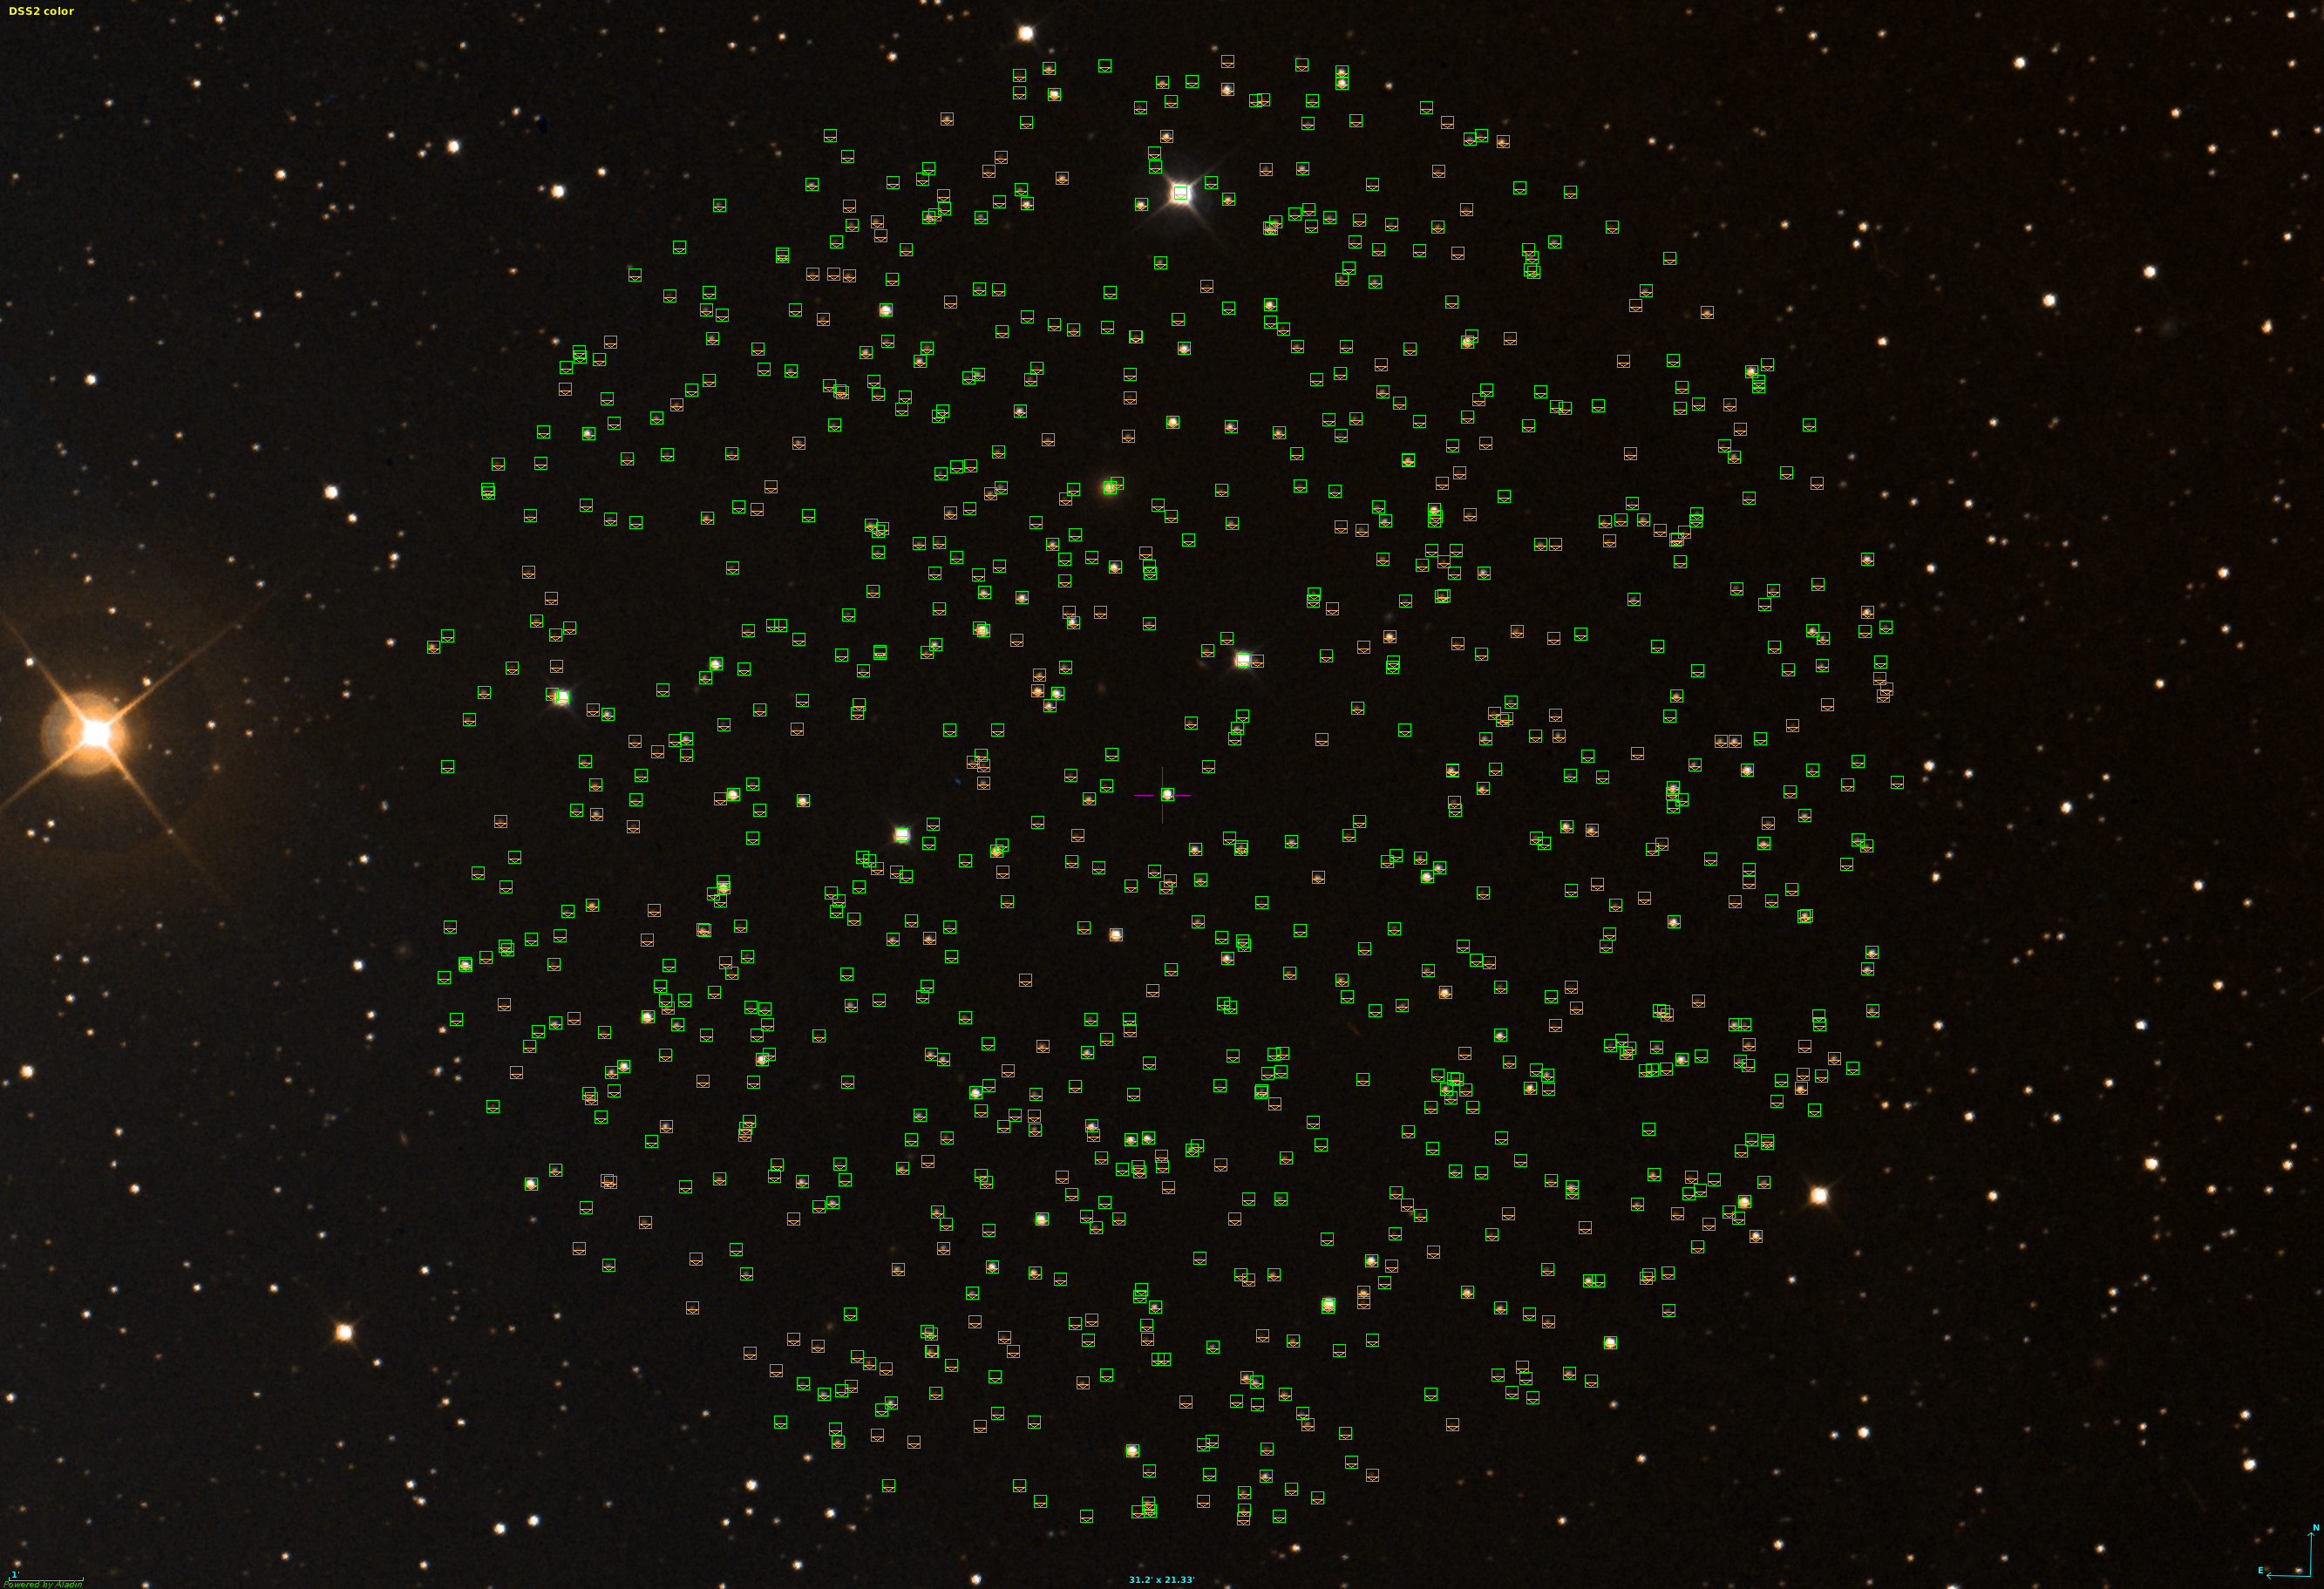
\includegraphics[width=0.49\linewidth]{img/gaia_180_20}
  \caption{Regiones de radio $10'$ de la galaxia seleccionadas para el ejercicio. A la izquierda, imagen de \ac{DSS2} de la región correspondiente a las coordenadas cercanas al plano galáctico $l=2.0,b=0$; a la derecha, región completamente alejada del plano galáctico $l=180,b=-20$. Imágenes obtenidas con el software \emph{Aladin}, las estrellas marcadas con cuadrados verdes corresponden a datos presentes en \emph{Gaia DR2}.}
\end{figure}

\begin{figure}
  \includegraphics[width=\linewidth]{img/ejercicio1_bprp_gmag}
\end{figure}

\begin{figure}
  \includegraphics[width=\linewidth]{img/ejercicio1_plx_gmag}
\end{figure}

\begin{figure}
  \includegraphics[width=\linewidth]{img/ejercicio1_pmra_pmde}
\end{figure}

\begin{figure}
  \includegraphics[width=0.49\linewidth]{img/ejercicio1_era_ede}
  \includegraphics[width=0.49\linewidth]{img/ejercicio1_era_ede_filtered}
\end{figure}

\section{Ejercicio 2}

\textbf{Carga los datos para las estrellas en torno al cúmulo abierto de las Pléyades (M45). Este es un cúmulo muy
cercano. Necesitarás tomar un radio grande (de, por lo menos, un grado). Intenta localizar el cúmulo en el
plano de los movimientos propios. Estudia su extensión en diferentes diagramas y selecciona un conjunto de
posibles miembros del cúmulo. Haz el mismo estudio para el cúmulo abierto problema que se ha asignado a tu grupo. Este cúmulo es más lejano y necesitarás tomar un radio entre $10'$ y $20'$. Una vez tengas una selección de miembros, identifica las estrellas evolucionadas que pertenecen al cúmulo. Dibuja el diagrama color/magnitud (en este caso, BP-RP/G) para los dos cúmulos. ¿Qué diferencias ves? ¿A qué puedes atribuirlo?}

\begin{figure}
  \includegraphics[width=0.49\linewidth]{img/pleyades}
  \includegraphics[width=0.49\linewidth]{img/pleyades_gaia}
  \caption{Región de $60'$ (1 grado) respecto al centro del cúmulo M45. A la izquierda, datos del catálogo \ac{DSS2} centrados en las coordenadas $l=166.56979, b=-23.52246$; a la derecha, la misma imagen con los datos de \emph{Gaia DR2} sobreimpuestos como cuadrados turquesas en la región dada. Imágenes obtenidas con el software \emph{Aladin}.}
\end{figure}

\begin{figure}
  \includegraphics[width=0.49\linewidth]{img/ejercicio2_m45_bprp_gmag}
  \includegraphics[width=0.49\linewidth]{img/ejercicio2_m45_bprp_gmag_14}
\end{figure}

\begin{figure}
  \includegraphics[width=0.49\linewidth]{img/ejercicio2_m45_pmde_pmra}
  \includegraphics[width=0.49\linewidth]{img/ejercicio2_m45_pmde_pmra_14}
\end{figure}

\begin{figure}
  \includegraphics[width=\linewidth]{img/ejercicio2_m45_plx_pmra}
\end{figure}

\begin{figure}
  \includegraphics[width=\linewidth]{img/ejercicio2_m45_plx_pmde}
\end{figure}

\begin{figure}
  \includegraphics[width=\linewidth]{img/m45_cumulo_def}
\end{figure}

\section{Ejercicio Opcional}

\textbf{Para las estrellas evolucionadas del cúmulo problema descarga datos fotométricos de diferentes catálogos y
estudia su distribución espectral de energía. ¿Qué te puede ser necesario?}


%%%%%%%%%%%%%%%%%%%%%%%%%%%%%%%%%%%%%%%%%%%%%%%%%%

%%%%%%%%%%%%%%%%%%%% REFERENCES %%%%%%%%%%%%%%%%%%

% The best way to enter references is to use BibTeX:

\bibliographystyle{mnras}
\bibliography{mnras} % if your bibtex file is called example.bib


%%%%%%%%%%%%%%%%%%%%%%%%%%%%%%%%%%%%%%%%%%%%%%%%%%

%%%%%%%%%%%%%%%%% APPENDICES %%%%%%%%%%%%%%%%%%%%%


%%%%%%%%%%%%%%%%%%%%%%%%%%%%%%%%%%%%%%%%%%%%%%%%%%


% Don't change these lines
\bsp	% typesetting comment
\label{lastpage}
\end{document}

% End of mnras_template.tex